% Options for packages loaded elsewhere
\PassOptionsToPackage{unicode}{hyperref}
\PassOptionsToPackage{hyphens}{url}
\documentclass[
]{article}
\usepackage[margin=0.75in]{geometry}
\usepackage{xcolor}
\usepackage{amsmath,amssymb}
\setcounter{secnumdepth}{5}
\usepackage{iftex}
\ifPDFTeX
  \usepackage[T1]{fontenc}
  \usepackage[utf8]{inputenc}
  \usepackage{textcomp} % provide euro and other symbols
\else % if luatex or xetex
  \usepackage{unicode-math} % this also loads fontspec
  \defaultfontfeatures{Scale=MatchLowercase}
  \defaultfontfeatures[\rmfamily]{Ligatures=TeX,Scale=1}
\fi
\usepackage{lmodern}
\ifPDFTeX\else
  % xetex/luatex font selection
\fi
% Use upquote if available, for straight quotes in verbatim environments
\IfFileExists{upquote.sty}{\usepackage{upquote}}{}
\IfFileExists{microtype.sty}{% use microtype if available
  \usepackage[]{microtype}
  \UseMicrotypeSet[protrusion]{basicmath} % disable protrusion for tt fonts
}{}
\makeatletter
\@ifundefined{KOMAClassName}{% if non-KOMA class
  \IfFileExists{parskip.sty}{%
    \usepackage{parskip}
  }{% else
    \setlength{\parindent}{0pt}
    \setlength{\parskip}{6pt plus 2pt minus 1pt}}
}{% if KOMA class
  \KOMAoptions{parskip=half}}
\makeatother
\usepackage{longtable,booktabs,array}
\newcounter{none} % for unnumbered tables
\usepackage{calc} % for calculating minipage widths
% Correct order of tables after \paragraph or \subparagraph
\usepackage{etoolbox}
\makeatletter
\patchcmd\longtable{\par}{\if@noskipsec\mbox{}\fi\par}{}{}
\makeatother
% Allow footnotes in longtable head/foot
\IfFileExists{footnotehyper.sty}{\usepackage{footnotehyper}}{\usepackage{footnote}}
\makesavenoteenv{longtable}
\usepackage{graphicx}
\makeatletter
\newsavebox\pandoc@box
\newcommand*\pandocbounded[1]{#1}%
% Set default figure placement to htbp
\def\fps@figure{htbp}
\makeatother
\setlength{\emergencystretch}{3em} % prevent overfull lines
\providecommand{\tightlist}{%
  \setlength{\itemsep}{0pt}\setlength{\parskip}{0pt}}
% Standard preamble for reslop analysis notes.
% Included via pandoc: --include-in-header=preamble.tex
% Do not edit per-analysis unless you have a specific reason.

% --- Graphics and floats ---
\usepackage{graphicx}
\usepackage{placeins}
\usepackage{float}
\usepackage{needspace}

% Default figure sizing: HEIGHT-based, not width-based.
%
% All figures are produced at figsize=(10,10) — square. But figures
% with colorbars (2D plots, correlation matrices) have extended width
% (e.g., 12x10 effective) due to the colorbar axes. Setting size by
% width makes these figures smaller than 1D plots at the same nominal
% width fraction, because the extra colorbar width eats into the budget.
%
% Setting size by HEIGHT avoids this: a 0.45\linewidth height gives
% consistent visual sizing regardless of colorbars, because the plot
% area height is always 10 inches. Two figures side-by-side at
% height=0.45\linewidth will have matching plot areas even if one has
% a colorbar and the other doesn't.
%
% We unset the default width and set height instead.
\setkeys{Gin}{height=0.45\linewidth,keepaspectratio}

% --- Caption formatting ---
% font=small keeps captions visually distinct from body text.
% Full column width for both figure and table captions.
\usepackage[font=small]{caption}

% --- Tables: prevent page splits ---
% Pandoc generates longtable by default, which splits across pages.
% We strongly discourage this by penalizing breaks inside floats.
% The typesetting agent should also convert longtables to regular
% table floats where the table fits on a single page.
\usepackage{longtable}
\setlength{\LTpre}{0pt}
\setlength{\LTpost}{0pt}

% --- Float placement (relaxed) ---
% LaTeX defaults are too conservative for figure-heavy technical docs.
% These settings allow up to 90% of a page to be floats, preventing
% overfull vbox warnings and figure cutoffs.
\renewcommand{\topfraction}{0.9}
\renewcommand{\bottomfraction}{0.9}
\renewcommand{\textfraction}{0.05}
\renewcommand{\floatpagefraction}{0.6}
\setcounter{topnumber}{3}
\setcounter{bottomnumber}{3}
\setcounter{totalnumber}{6}

% --- Paragraph and page breaking ---
% Prevent widows and orphans (single lines at top/bottom of page).
\widowpenalty=10000
\clubpenalty=10000
% Allow ragged page bottoms rather than stretching vertical glue
% (which creates ugly spacing between paragraphs).
\raggedbottom
\usepackage{bookmark}
\IfFileExists{xurl.sty}{\usepackage{xurl}}{} % add URL line breaks if available
\urlstyle{same}
\hypersetup{
  pdftitle={CMS Open Data H to tau tau Search: Phase 4c Audit-Corrected Observed Results},
  pdfauthor={Analysis my\_analysis},
  hidelinks,
  pdfcreator={LaTeX via pandoc}}

\title{CMS Open Data H to tau tau Search: Phase 4c Audit-Corrected
Observed Results}
\author{Analysis my\_analysis}
\date{2026-06-02}

\begin{document}
\maketitle

{
\setcounter{tocdepth}{3}
\tableofcontents
}
\needspace{4\baselineskip}
\section*{Change Log}\label{change-log}
\addcontentsline{toc}{section}{Change Log}

\textbf{Phase 4c v2 audit correction}

\begin{itemize}
\tightlist
\item
  Added a same-sign data-driven QCD/fake background estimate.
\item
  Added multivariate data/MC input reweighting derived in
  validation/control regions before classifier training.
\item
  Promoted the calibrated categorized score model to the primary
  observed result.
\item
  Widened DY/Z normalization to reflect the absence of embedding and EWK
  Z reduced samples.
\end{itemize}

\needspace{4\baselineskip}
\FloatBarrier
\section{Phase 4c Observed Inference: Audit-Corrected Full
Data}\label{phase-4c-observed-inference-audit-corrected-full-data}

\needspace{4\baselineskip}
\subsection{Summary}\label{summary}

Phase 4c has been updated after the audit of the large expected versus
observed discrepancy. The problem was physics modelling: the original
score-template fit omitted a reducible QCD/fake-tau component, used
background MC before correcting large data/MC input-shape differences,
and carried too restrictive a DY/Z normalization model for a reduced
sample without embedding or EWK Z simulation.

The primary observed result is therefore the calibrated
trained-discriminator fit in the same VBF, boosted, and zero-jet
categories. The classifier is trained only on MC, but the background MC
receives a multivariate data/MC input reweighting derived before
training in W high-mT, same-sign, Z-rich, and top/b-tag
validation/control regions. The primary score model also includes the
same-sign data-driven QCD/fake template and wider DY/Z normalization
nuisance terms. Visible mass and add-MET mass are retained only as
cross-checks.

\needspace{4\baselineskip}
\subsection{W and QCD Control Inputs}\label{w-and-qcd-control-inputs}

The full-data W+jets scale from the high-mT control region is
\texttt{0.8528\ ±\ 0.0370}. The VBF background control scale from the
VBF-like top-btag non-signal region is \texttt{0.5571\ ±\ 0.0515}; it is
applied only to MC backgrounds in the VBF fit category. This addresses
the large VBF data/MC overprediction seen in the original observed
templates without changing the signal normalization or the
boosted/zero-jet categories. The same-sign QCD/fake estimate uses data
minus non-QCD MC in the same-sign low-mT region and a transfer factor
measured in the lowest fitted-observable bin. For the primary
calibrated-score model this factor is \texttt{0.0204\ ±\ 0.2533}. For
the visible-mass cross-check it is \texttt{0.0087\ ±\ 0.4828}. For the
add-MET mass cross-check it is \texttt{0.2654\ ±\ 1.0277}.

\needspace{0.4\textheight}
\begin{figure}[htbp]
\centering
\pandocbounded{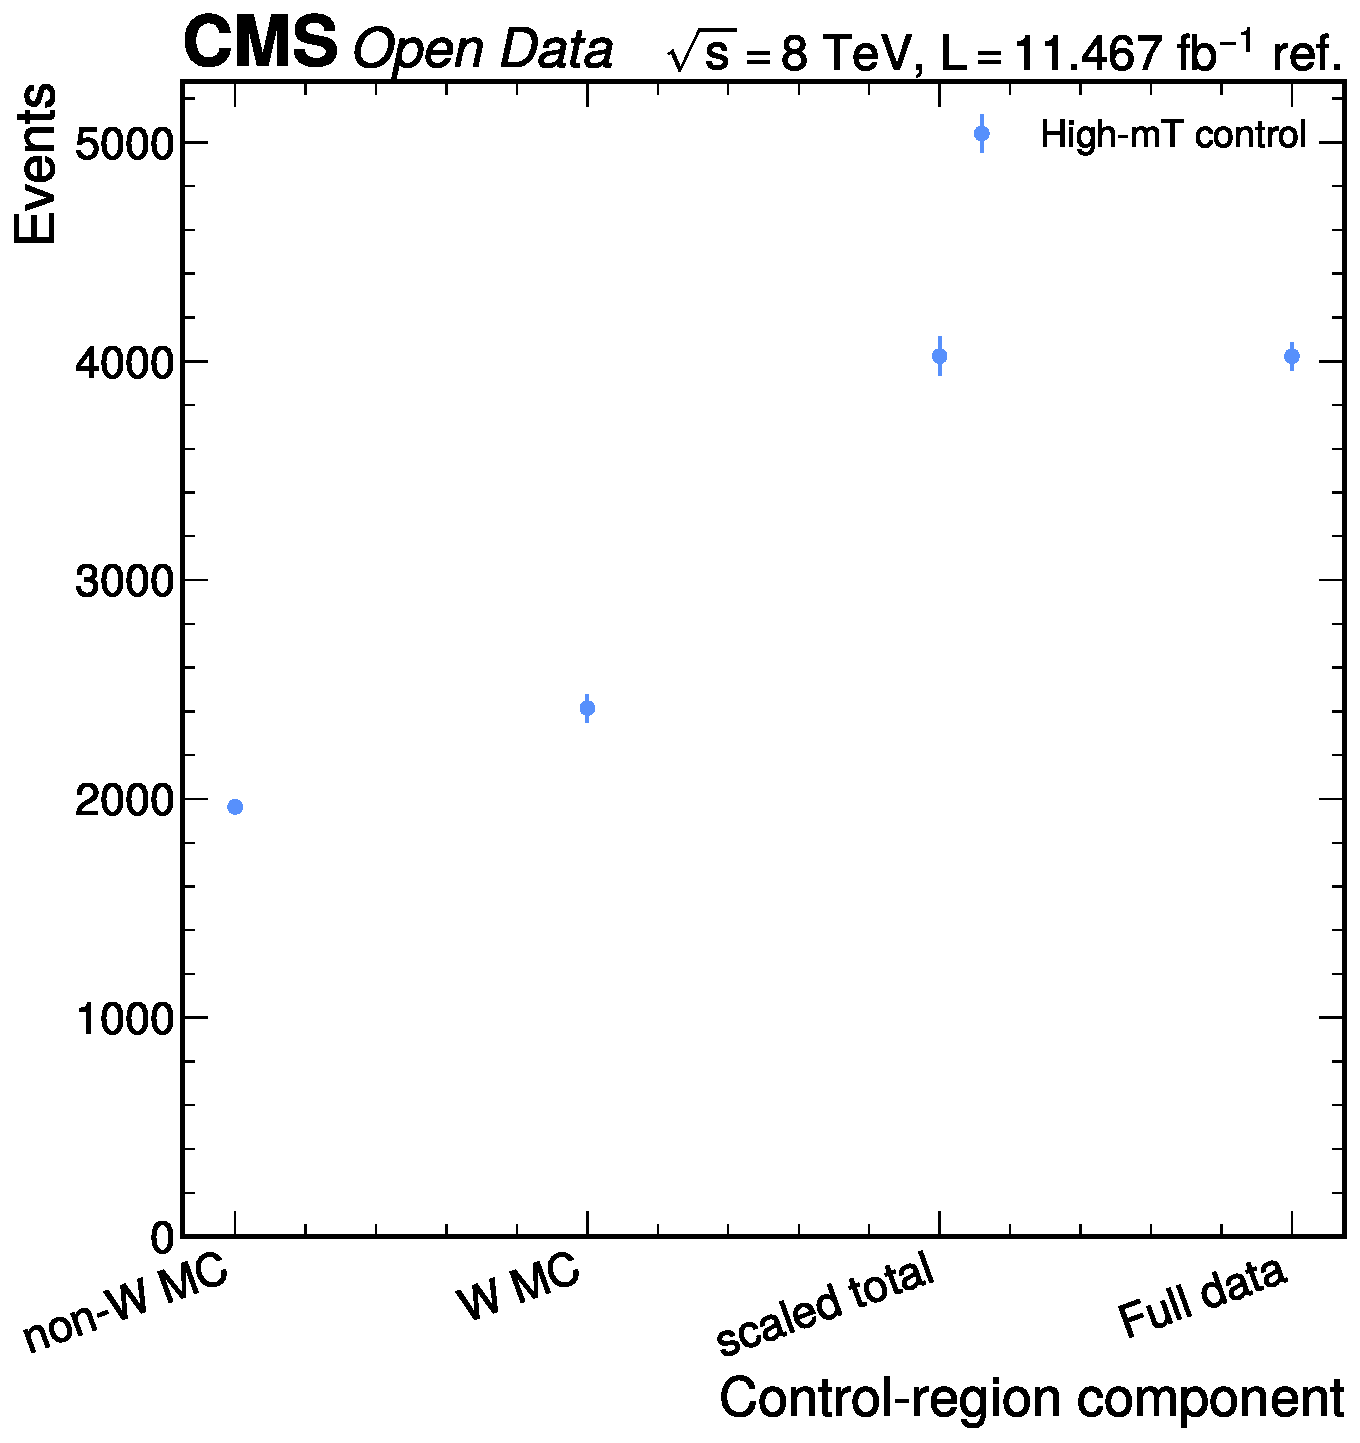
\includegraphics[height=0.35\textheight,width=\linewidth,keepaspectratio,alt={Full high-mT W control comparison. The figure shows non-W MC, nominal W MC, the scaled control-region prediction, and full data in the control region. The scale is derived outside the signal region and then propagated into the observed workspaces.}]{figures/w_highmt_scale_full.pdf}}
\caption{Full high-mT W control comparison. The figure shows non-W MC,
nominal W MC, the scaled control-region prediction, and full data in the
control region. The scale is derived outside the signal region and then
propagated into the observed workspaces.}\label{fig:p4c-wcr}
\end{figure}

\needspace{4\baselineskip}
\subsection{Primary Calibrated-Score
Result}\label{primary-calibrated-score-result}

{\def\LTcaptype{none} % do not increment counter
\vspace{1em}
\begin{table}[htbp]
\centering
\small
\begin{tabular}{@{}
>{\raggedright\arraybackslash}p{(\linewidth - 12\tabcolsep) * \real{0.1111}}
  >{\raggedleft\arraybackslash}p{(\linewidth - 12\tabcolsep) * \real{0.1481}}
  >{\raggedleft\arraybackslash}p{(\linewidth - 12\tabcolsep) * \real{0.1481}}
  >{\raggedleft\arraybackslash}p{(\linewidth - 12\tabcolsep) * \real{0.1481}}
  >{\raggedleft\arraybackslash}p{(\linewidth - 12\tabcolsep) * \real{0.1481}}
  >{\raggedleft\arraybackslash}p{(\linewidth - 12\tabcolsep) * \real{0.1481}}
  >{\raggedleft\arraybackslash}p{(\linewidth - 12\tabcolsep) * \real{0.1481}}@{}}
\toprule\noalign{}
\begin{minipage}[b]{\linewidth}\raggedright
Category
\end{minipage} & \begin{minipage}[b]{\linewidth}\raggedleft
Data
\end{minipage} & \begin{minipage}[b]{\linewidth}\raggedleft
Background
\end{minipage} & \begin{minipage}[b]{\linewidth}\raggedleft
QCD/fake
\end{minipage} & \begin{minipage}[b]{\linewidth}\raggedleft
Data/background
\end{minipage} & \begin{minipage}[b]{\linewidth}\raggedleft
Chi2/ndf
\end{minipage} & \begin{minipage}[b]{\linewidth}\raggedleft
Max abs pull
\end{minipage} \\
\midrule\noalign{}
vbf & 79 & 60.17 & 0.36 & 1.313 & 1.513 & 2.36 \\
boosted & 2213 & 2115.53 & 5.64 & 1.046 & 1.904 & 2.63 \\
zero\_jet & 8466 & 14047.12 & 22.93 & 0.603 & 4.025 & 3.22 \\
\end{tabular}
\end{table}
}

The primary calibrated-score fit gives \texttt{mu\_hat\ =\ 38.3802}, an
observed 95\% CLs limit \texttt{mu\ \textless{}\ 50.0000}, and a
diagnostic \texttt{q0} value \texttt{Z\ =\ 12.4698}. The median expected
limit from the same corrected workspace is \texttt{1.9735}.

\needspace{0.4\textheight}
\begin{figure}[htbp]
\centering
\pandocbounded{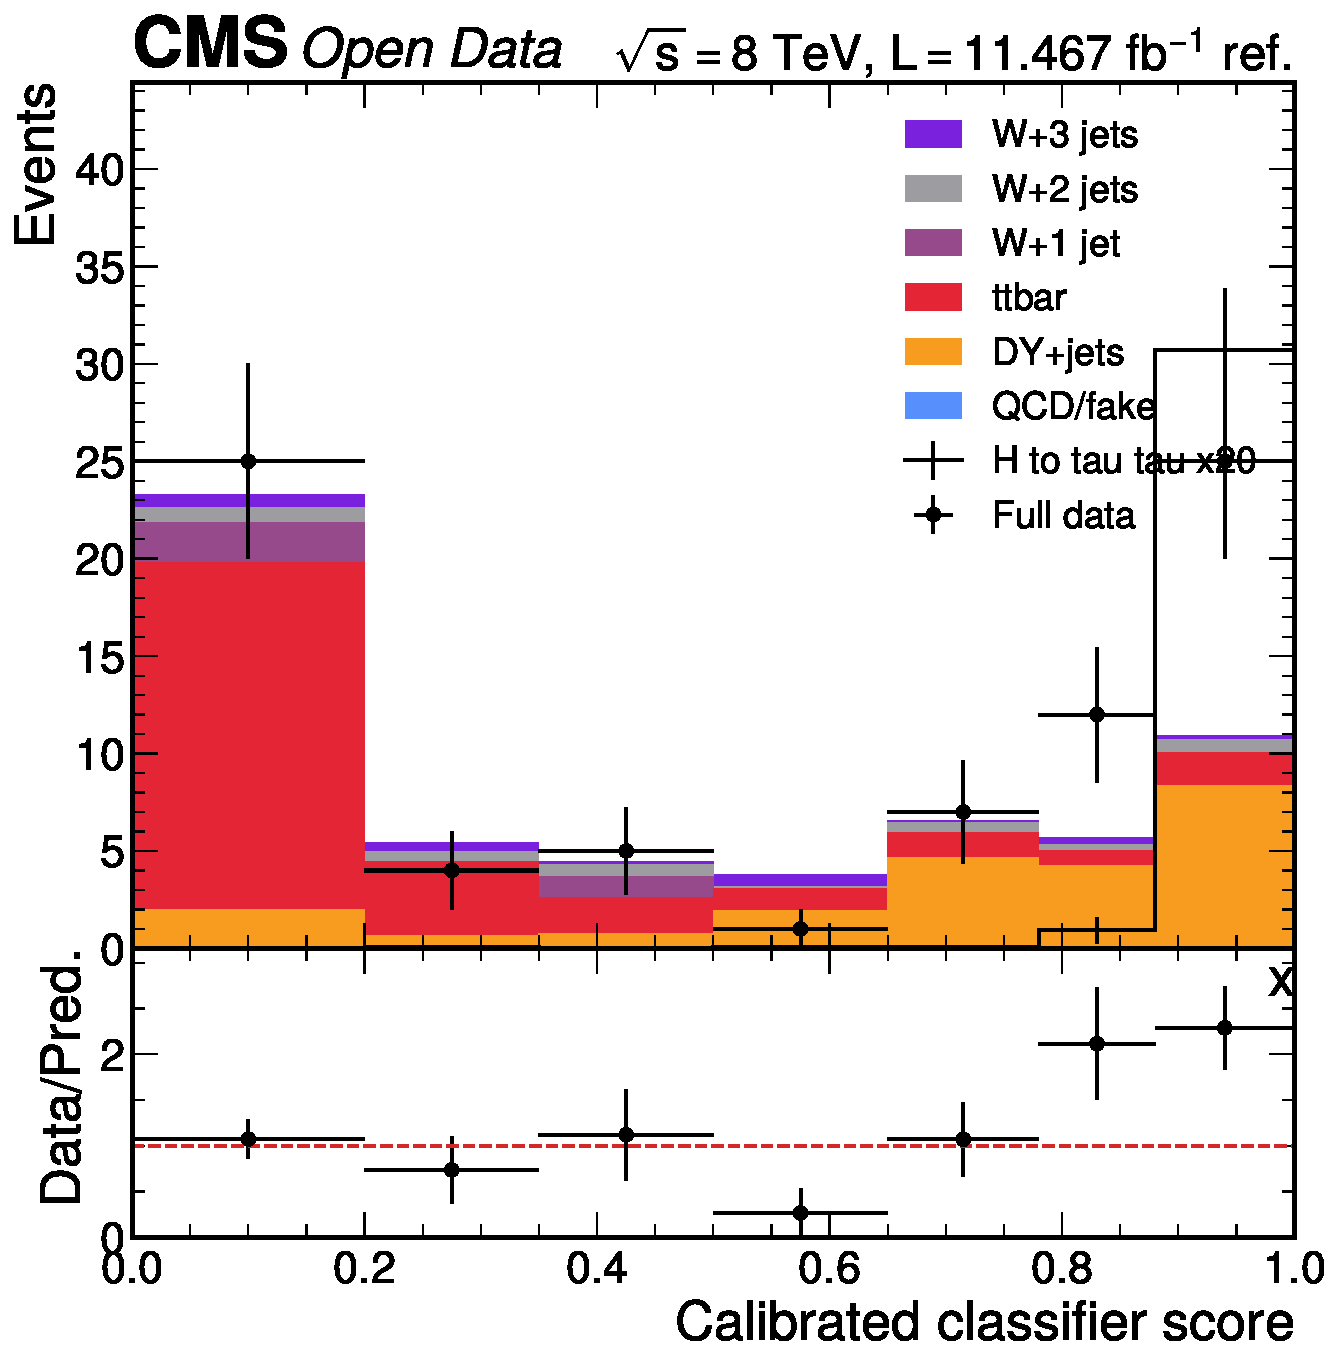
\includegraphics[height=0.35\textheight,width=\linewidth,keepaspectratio,alt={Primary calibrated-score validation in the VBF category. The plot compares localized Run2012B/C TauPlusX data to the calibrated score model after pre-training multivariate input reweighting, wider DY/Z normalization, and same-sign QCD/fake correction. This category remains statistically limited but is included in the simultaneous primary fit.}]{figures/observed_primary_score_vbf.pdf}}
\caption{Primary calibrated-score validation in the VBF category. The
plot compares localized Run2012B/C TauPlusX data to the calibrated score
model after pre-training multivariate input reweighting, wider DY/Z
normalization, and same-sign QCD/fake correction. This category remains
statistically limited but is included in the simultaneous primary
fit.}\label{fig:p4c-primary-vbf}
\end{figure}

\needspace{0.4\textheight}
\begin{figure}[htbp]
\centering
\pandocbounded{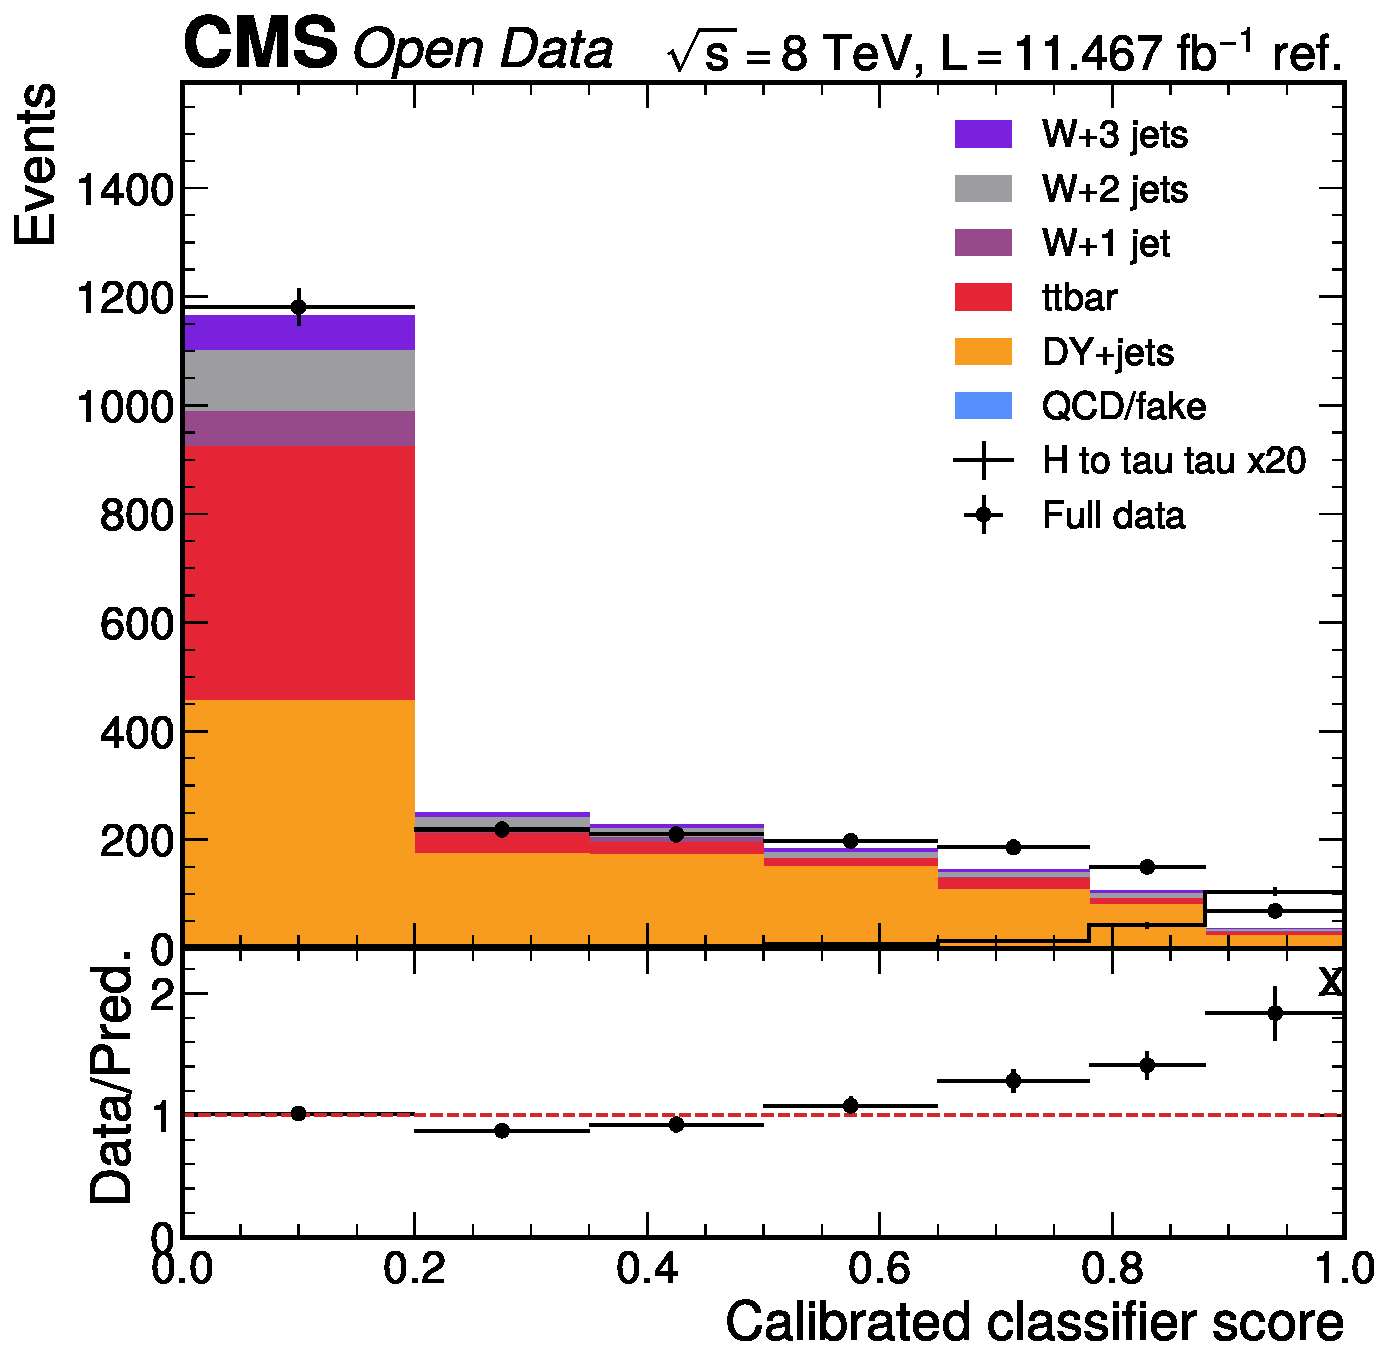
\includegraphics[height=0.35\textheight,width=\linewidth,keepaspectratio,alt={Primary calibrated-score validation in the boosted category. The plot compares full data to the calibrated score model with the W high-mT scale and same-sign QCD/fake template. This category is used in the final observed fit.}]{figures/observed_primary_score_boosted.pdf}}
\caption{Primary calibrated-score validation in the boosted category.
The plot compares full data to the calibrated score model with the W
high-mT scale and same-sign QCD/fake template. This category is used in
the final observed fit.}\label{fig:p4c-primary-boosted}
\end{figure}

\needspace{0.4\textheight}
\begin{figure}[htbp]
\centering
\pandocbounded{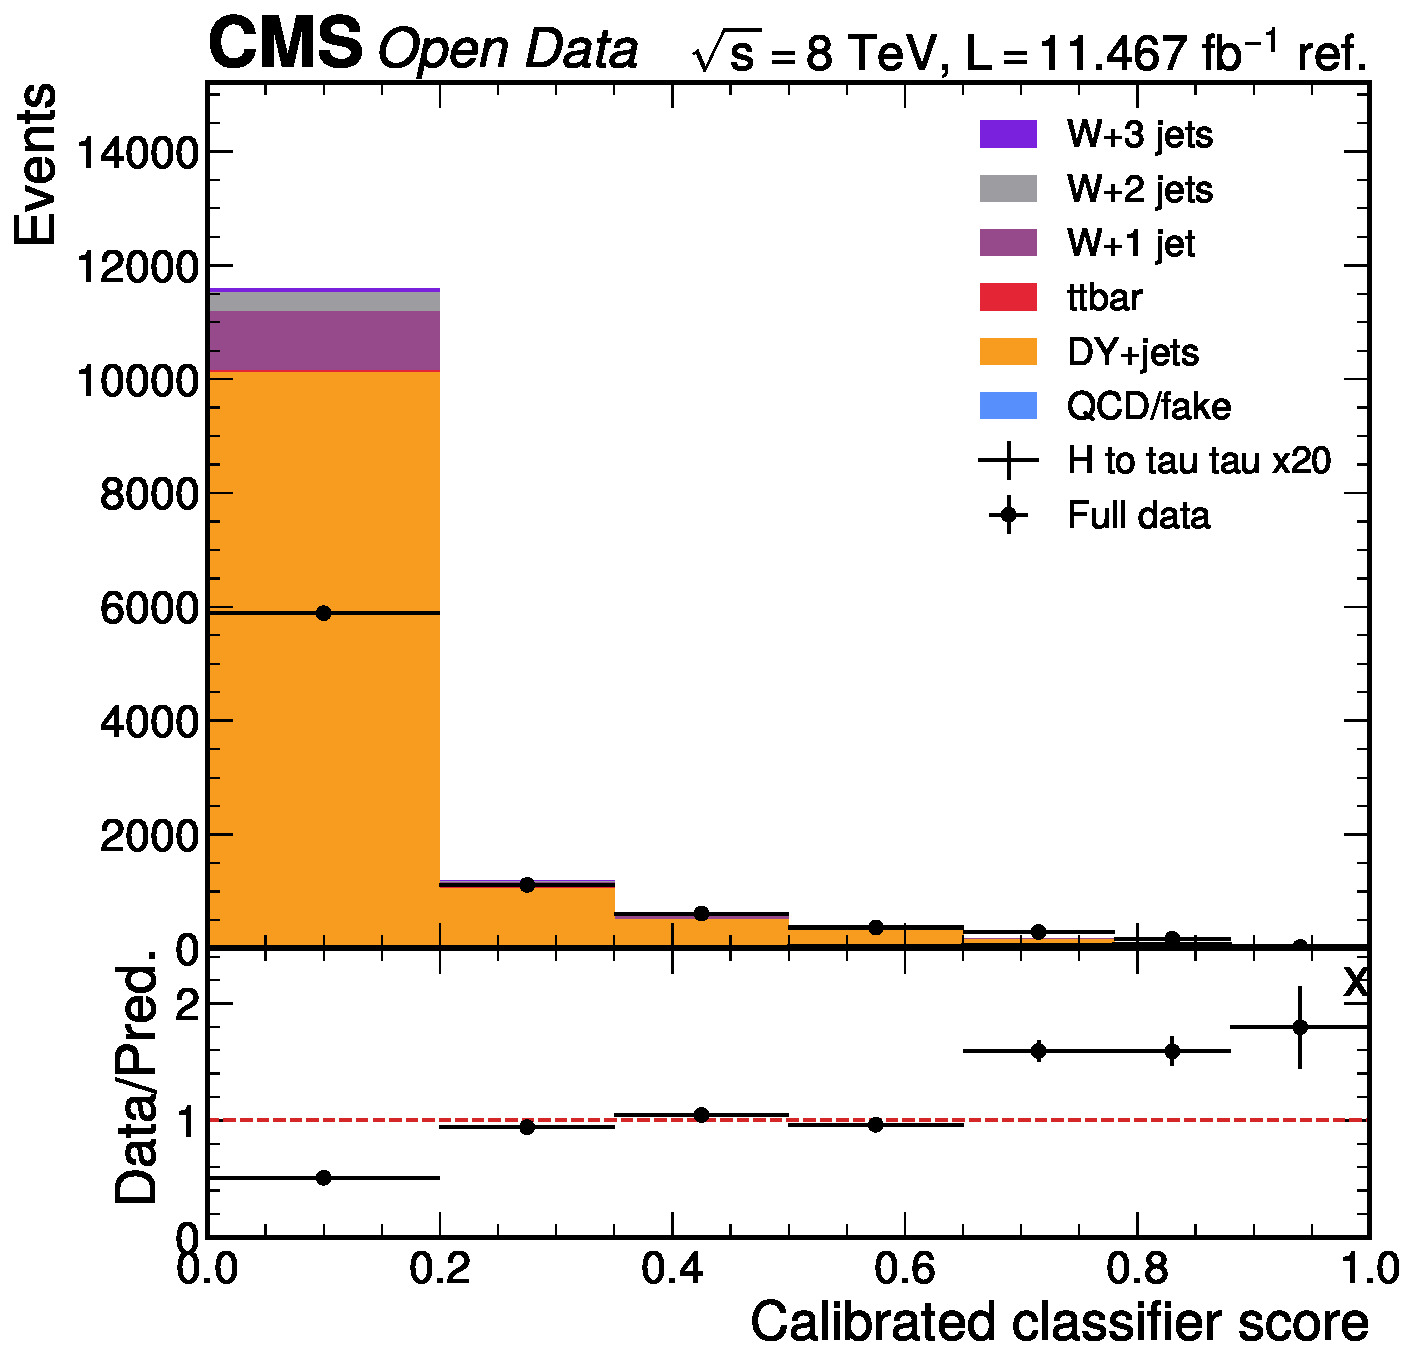
\includegraphics[height=0.35\textheight,width=\linewidth,keepaspectratio,alt={Primary calibrated-score validation in the zero-jet category. The zero-jet normalization is stabilized by the same-sign QCD/fake estimate and the background input reweighting. This category contributes the largest data statistics to the primary simultaneous fit.}]{figures/observed_primary_score_zero_jet.pdf}}
\caption{Primary calibrated-score validation in the zero-jet category.
The zero-jet normalization is stabilized by the same-sign QCD/fake
estimate and the background input reweighting. This category contributes
the largest data statistics to the primary simultaneous
fit.}\label{fig:p4c-primary-zero}
\end{figure}

\needspace{4\baselineskip}
\subsection{Add-MET Mass Cross-Check}\label{add-met-mass-cross-check}

{\def\LTcaptype{none} % do not increment counter
\vspace{1em}
\begin{table}[htbp]
\centering
\small
\begin{tabular}{@{}
>{\raggedright\arraybackslash}p{(\linewidth - 12\tabcolsep) * \real{0.1111}}
  >{\raggedleft\arraybackslash}p{(\linewidth - 12\tabcolsep) * \real{0.1481}}
  >{\raggedleft\arraybackslash}p{(\linewidth - 12\tabcolsep) * \real{0.1481}}
  >{\raggedleft\arraybackslash}p{(\linewidth - 12\tabcolsep) * \real{0.1481}}
  >{\raggedleft\arraybackslash}p{(\linewidth - 12\tabcolsep) * \real{0.1481}}
  >{\raggedleft\arraybackslash}p{(\linewidth - 12\tabcolsep) * \real{0.1481}}
  >{\raggedleft\arraybackslash}p{(\linewidth - 12\tabcolsep) * \real{0.1481}}@{}}
\toprule\noalign{}
\begin{minipage}[b]{\linewidth}\raggedright
Category
\end{minipage} & \begin{minipage}[b]{\linewidth}\raggedleft
Data
\end{minipage} & \begin{minipage}[b]{\linewidth}\raggedleft
Background
\end{minipage} & \begin{minipage}[b]{\linewidth}\raggedleft
QCD/fake
\end{minipage} & \begin{minipage}[b]{\linewidth}\raggedleft
Data/background
\end{minipage} & \begin{minipage}[b]{\linewidth}\raggedleft
Chi2/ndf
\end{minipage} & \begin{minipage}[b]{\linewidth}\raggedleft
Max abs pull
\end{minipage} \\
\midrule\noalign{}
vbf & 77 & 62.39 & 5.37 & 1.234 & 0.326 & 0.96 \\
boosted & 2177 & 2146.55 & 72.74 & 1.014 & 0.193 & 0.72 \\
zero\_jet & 8448 & 14313.61 & 299.76 & 0.590 & 4.707 & 4.07 \\
\end{tabular}
\end{table}
}

The simultaneous add-MET mass fit gives \texttt{mu\_hat\ =\ 39.1162}, an
observed 95\% CLs limit \texttt{mu\ \textless{}\ 50.0000}, and
\texttt{Z\ =\ 4.2223}. This fit uses the same categories and nuisance
model as the calibrated-score primary fit, but it is kept as a separate
cross-check rather than replacing the trained-discriminator result.

\needspace{0.4\textheight}
\begin{figure}[htbp]
\centering
\pandocbounded{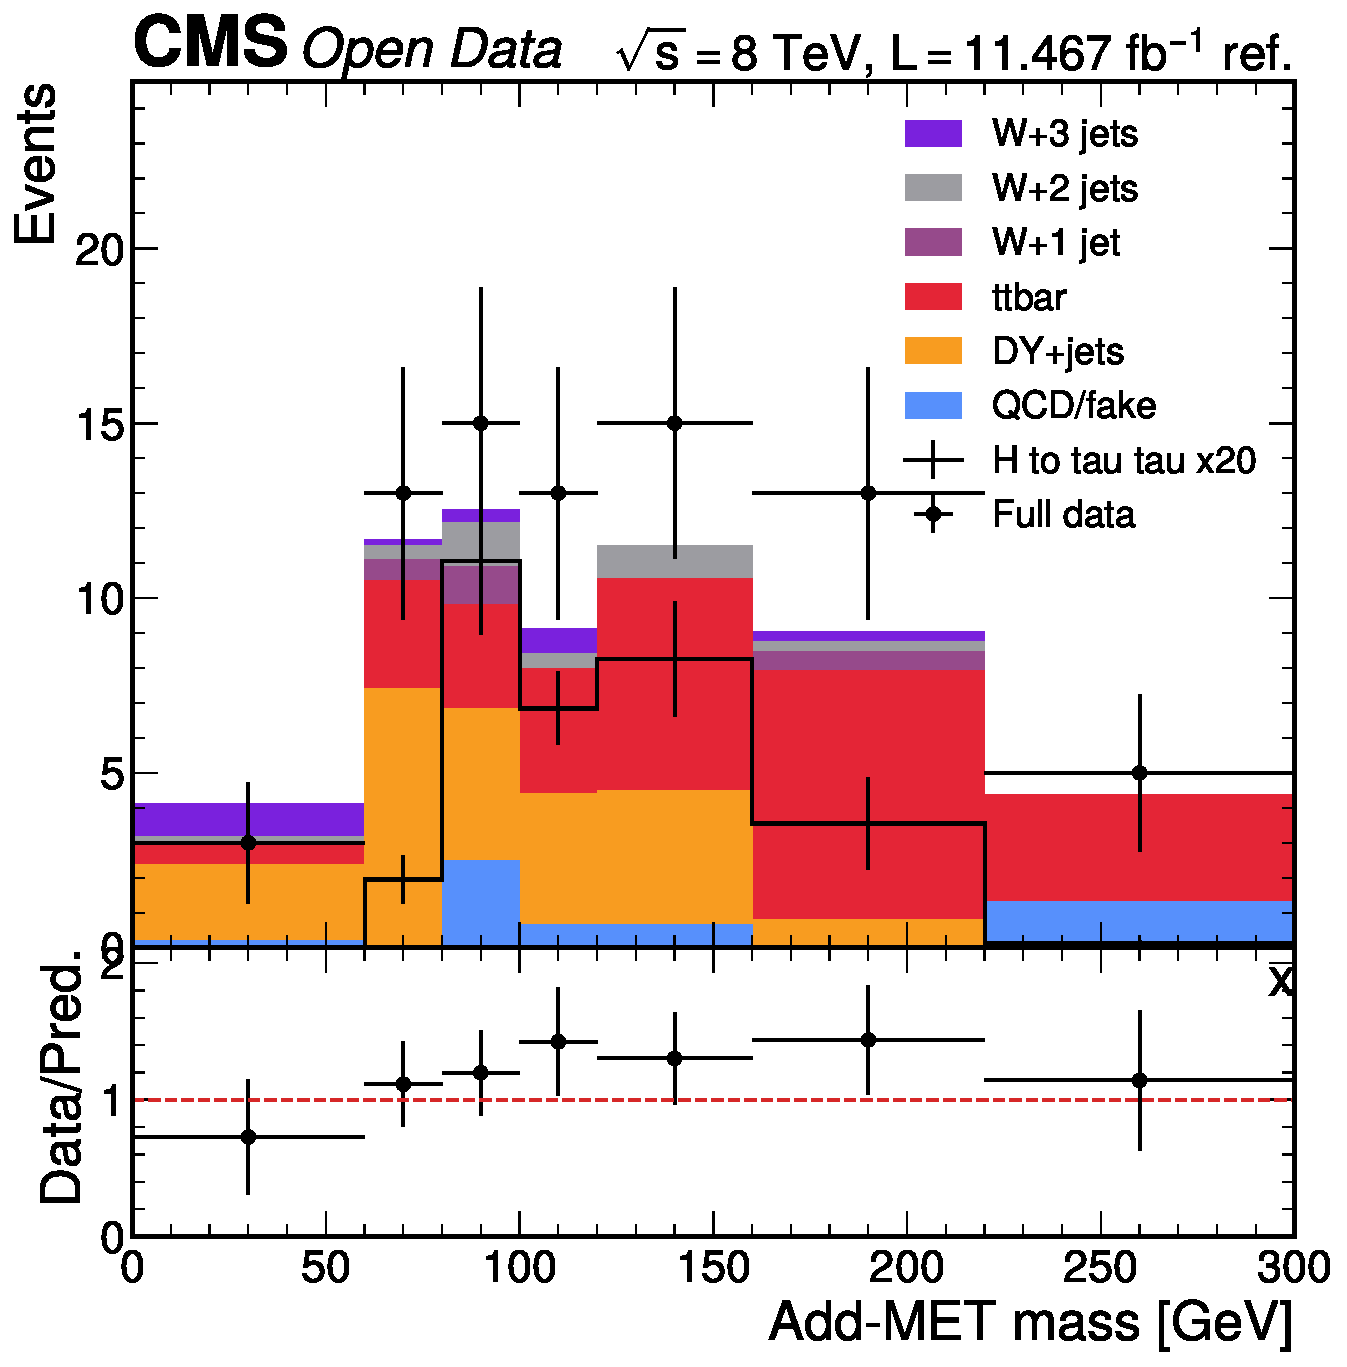
\includegraphics[height=0.35\textheight,width=\linewidth,keepaspectratio,alt={Add-MET mass validation in the VBF category. The plot compares full data to the QCD-corrected add-MET mass model in the VBF category. It uses the same W control scale, VBF background control scale, and same-sign QCD/fake transfer machinery as the calibrated-score primary model.}]{figures/observed_addmet_vbf.pdf}}
\caption{Add-MET mass validation in the VBF category. The plot compares
full data to the QCD-corrected add-MET mass model in the VBF category.
It uses the same W control scale, VBF background control scale, and
same-sign QCD/fake transfer machinery as the calibrated-score primary
model.}\label{fig:p4c-addmet-vbf}
\end{figure}

\needspace{0.4\textheight}
\begin{figure}[htbp]
\centering
\pandocbounded{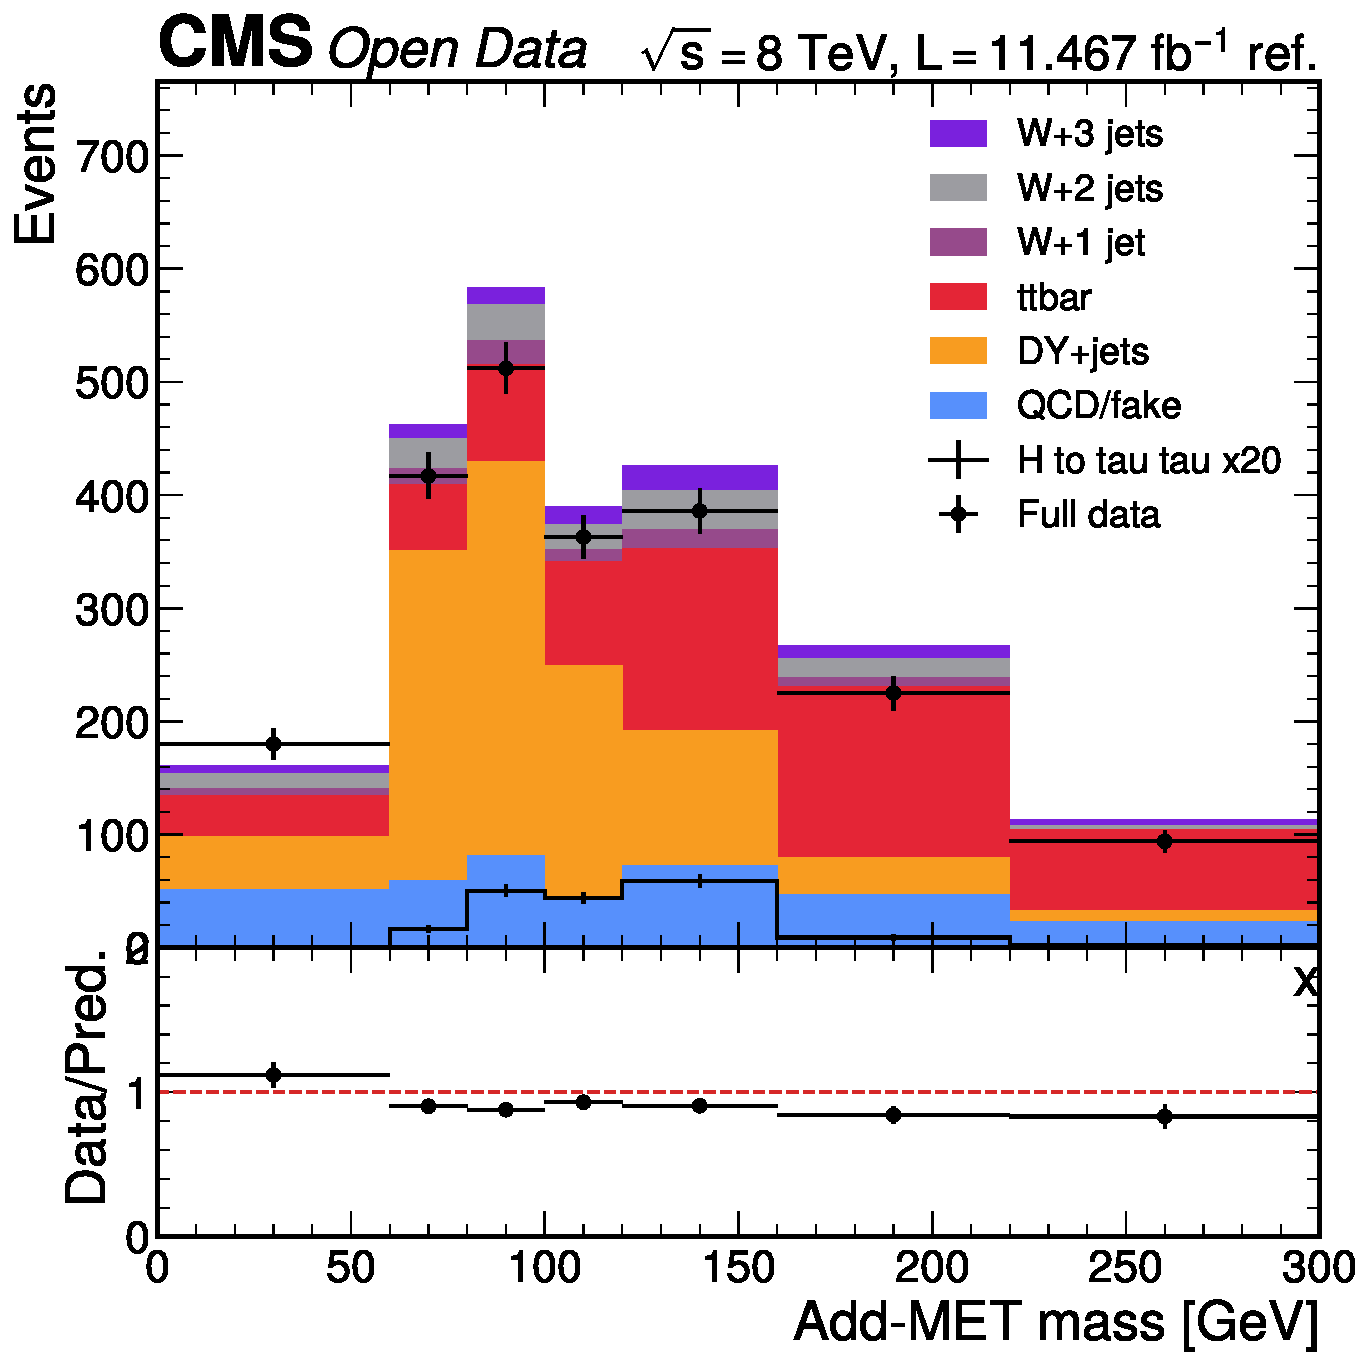
\includegraphics[height=0.35\textheight,width=\linewidth,keepaspectratio,alt={Add-MET mass validation in the boosted category. The plot compares full data to the add-MET mass model in the boosted category. The add-MET result is stored as an explicit Phase 4c cross-check output for downstream documentation.}]{figures/observed_addmet_boosted.pdf}}
\caption{Add-MET mass validation in the boosted category. The plot
compares full data to the add-MET mass model in the boosted category.
The add-MET result is stored as an explicit Phase 4c cross-check output
for downstream documentation.}\label{fig:p4c-addmet-boosted}
\end{figure}

\needspace{0.4\textheight}
\begin{figure}[htbp]
\centering
\pandocbounded{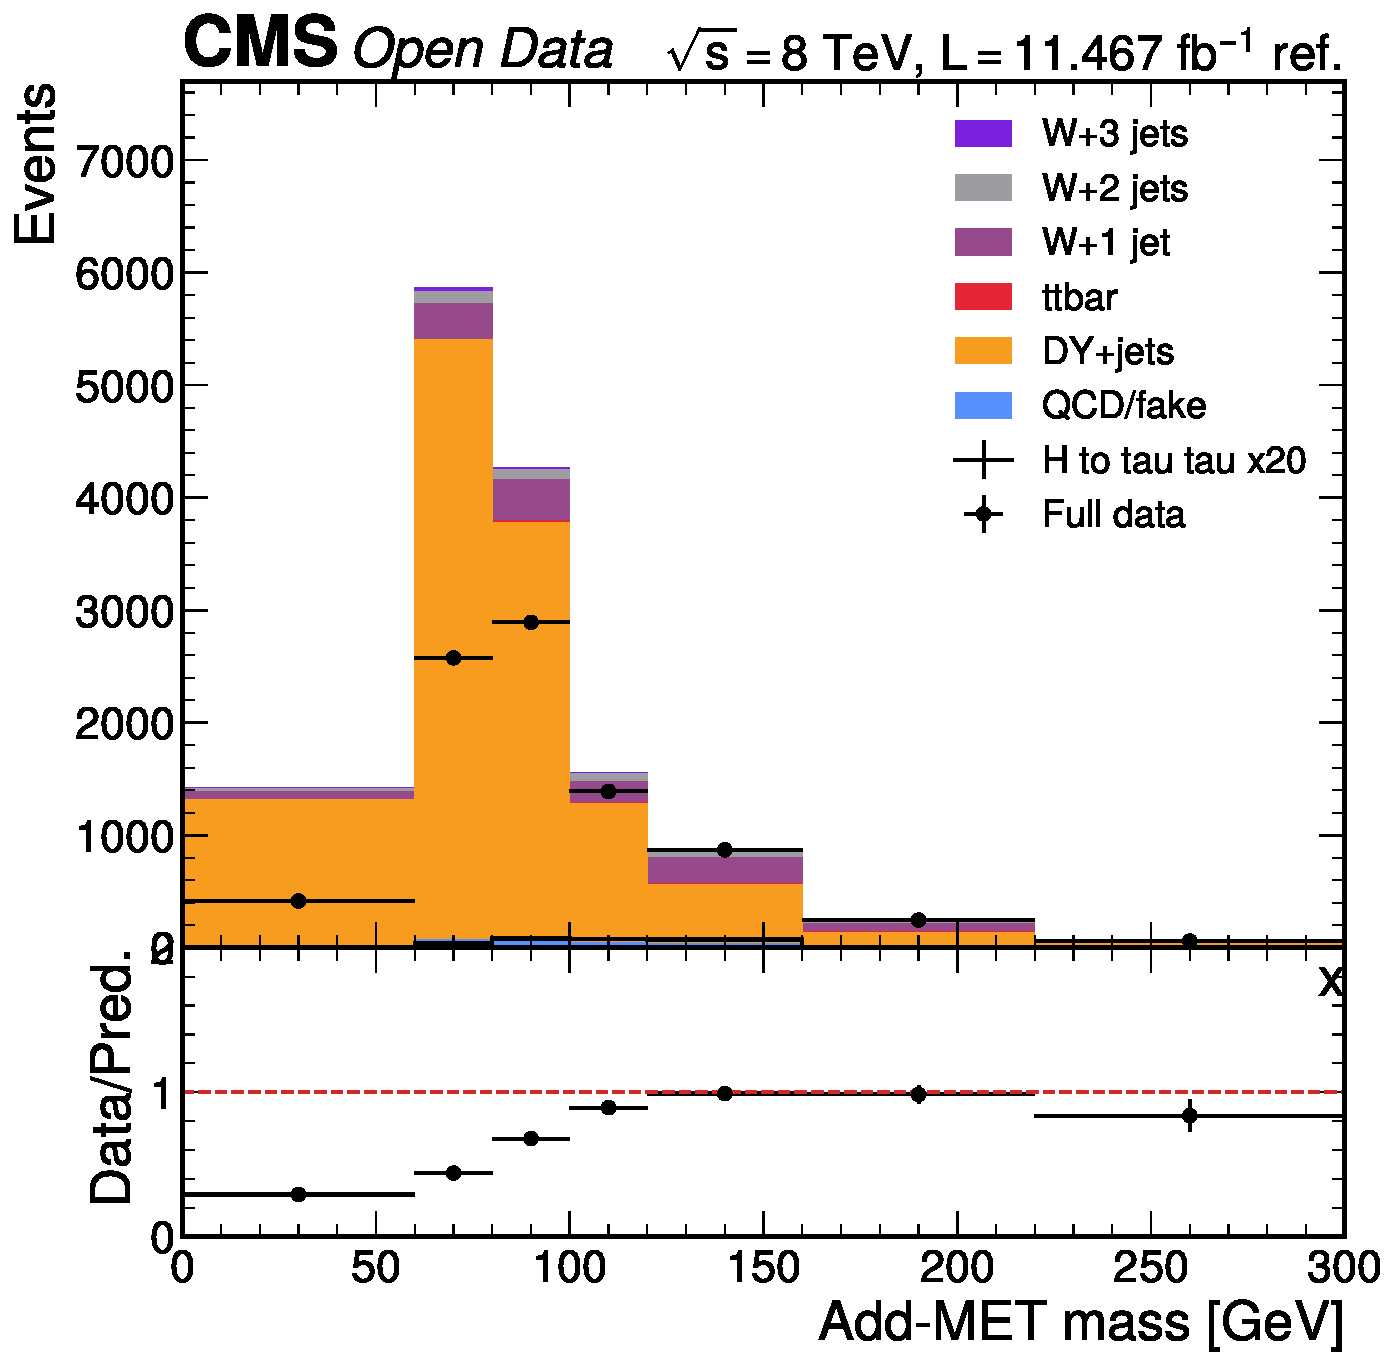
\includegraphics[height=0.35\textheight,width=\linewidth,keepaspectratio,alt={Add-MET mass validation in the zero-jet category. The plot compares full data to the add-MET mass model in the zero-jet category. This validates the alternative reconstructed-MET observable without modifying the primary calibrated-score fit.}]{figures/observed_addmet_zero_jet.pdf}}
\caption{Add-MET mass validation in the zero-jet category. The plot
compares full data to the add-MET mass model in the zero-jet category.
This validates the alternative reconstructed-MET observable without
modifying the primary calibrated-score fit.}\label{fig:p4c-addmet-zero}
\end{figure}

\needspace{4\baselineskip}
\subsection{Visible-Mass Cross-Check}\label{visible-mass-cross-check}

{\def\LTcaptype{none} % do not increment counter
\vspace{1em}
\begin{table}[htbp]
\centering
\small
\begin{tabular}{@{}
>{\raggedright\arraybackslash}p{(\linewidth - 12\tabcolsep) * \real{0.1111}}
  >{\raggedleft\arraybackslash}p{(\linewidth - 12\tabcolsep) * \real{0.1481}}
  >{\raggedleft\arraybackslash}p{(\linewidth - 12\tabcolsep) * \real{0.1481}}
  >{\raggedleft\arraybackslash}p{(\linewidth - 12\tabcolsep) * \real{0.1481}}
  >{\raggedleft\arraybackslash}p{(\linewidth - 12\tabcolsep) * \real{0.1481}}
  >{\raggedleft\arraybackslash}p{(\linewidth - 12\tabcolsep) * \real{0.1481}}
  >{\raggedleft\arraybackslash}p{(\linewidth - 12\tabcolsep) * \real{0.1481}}@{}}
\toprule\noalign{}
\begin{minipage}[b]{\linewidth}\raggedright
Category
\end{minipage} & \begin{minipage}[b]{\linewidth}\raggedleft
Data
\end{minipage} & \begin{minipage}[b]{\linewidth}\raggedleft
Background
\end{minipage} & \begin{minipage}[b]{\linewidth}\raggedleft
QCD/fake
\end{minipage} & \begin{minipage}[b]{\linewidth}\raggedleft
Data/background
\end{minipage} & \begin{minipage}[b]{\linewidth}\raggedleft
Chi2/ndf
\end{minipage} & \begin{minipage}[b]{\linewidth}\raggedleft
Max abs pull
\end{minipage} \\
\midrule\noalign{}
vbf & 78 & 57.72 & 0.17 & 1.351 & 1.189 & 2.07 \\
boosted & 2183 & 2085.76 & 2.41 & 1.047 & 0.846 & 1.77 \\
zero\_jet & 8451 & 14022.53 & 9.83 & 0.603 & 2.823 & 4.01 \\
\end{tabular}
\end{table}
}

The visible-mass cross-check gives \texttt{mu\_hat\ =\ 50.0000}, an
observed 95\% CLs limit \texttt{mu\ \textless{}\ 50.0000}, and
\texttt{Z\ =\ 5.4113}. The visible-mass fit is not the primary result in
this update because the trained calibrated score gives the stronger
expected sensitivity after the input-reweighting and DY/QCD corrections.

\needspace{0.4\textheight}
\begin{figure}[htbp]
\centering
\pandocbounded{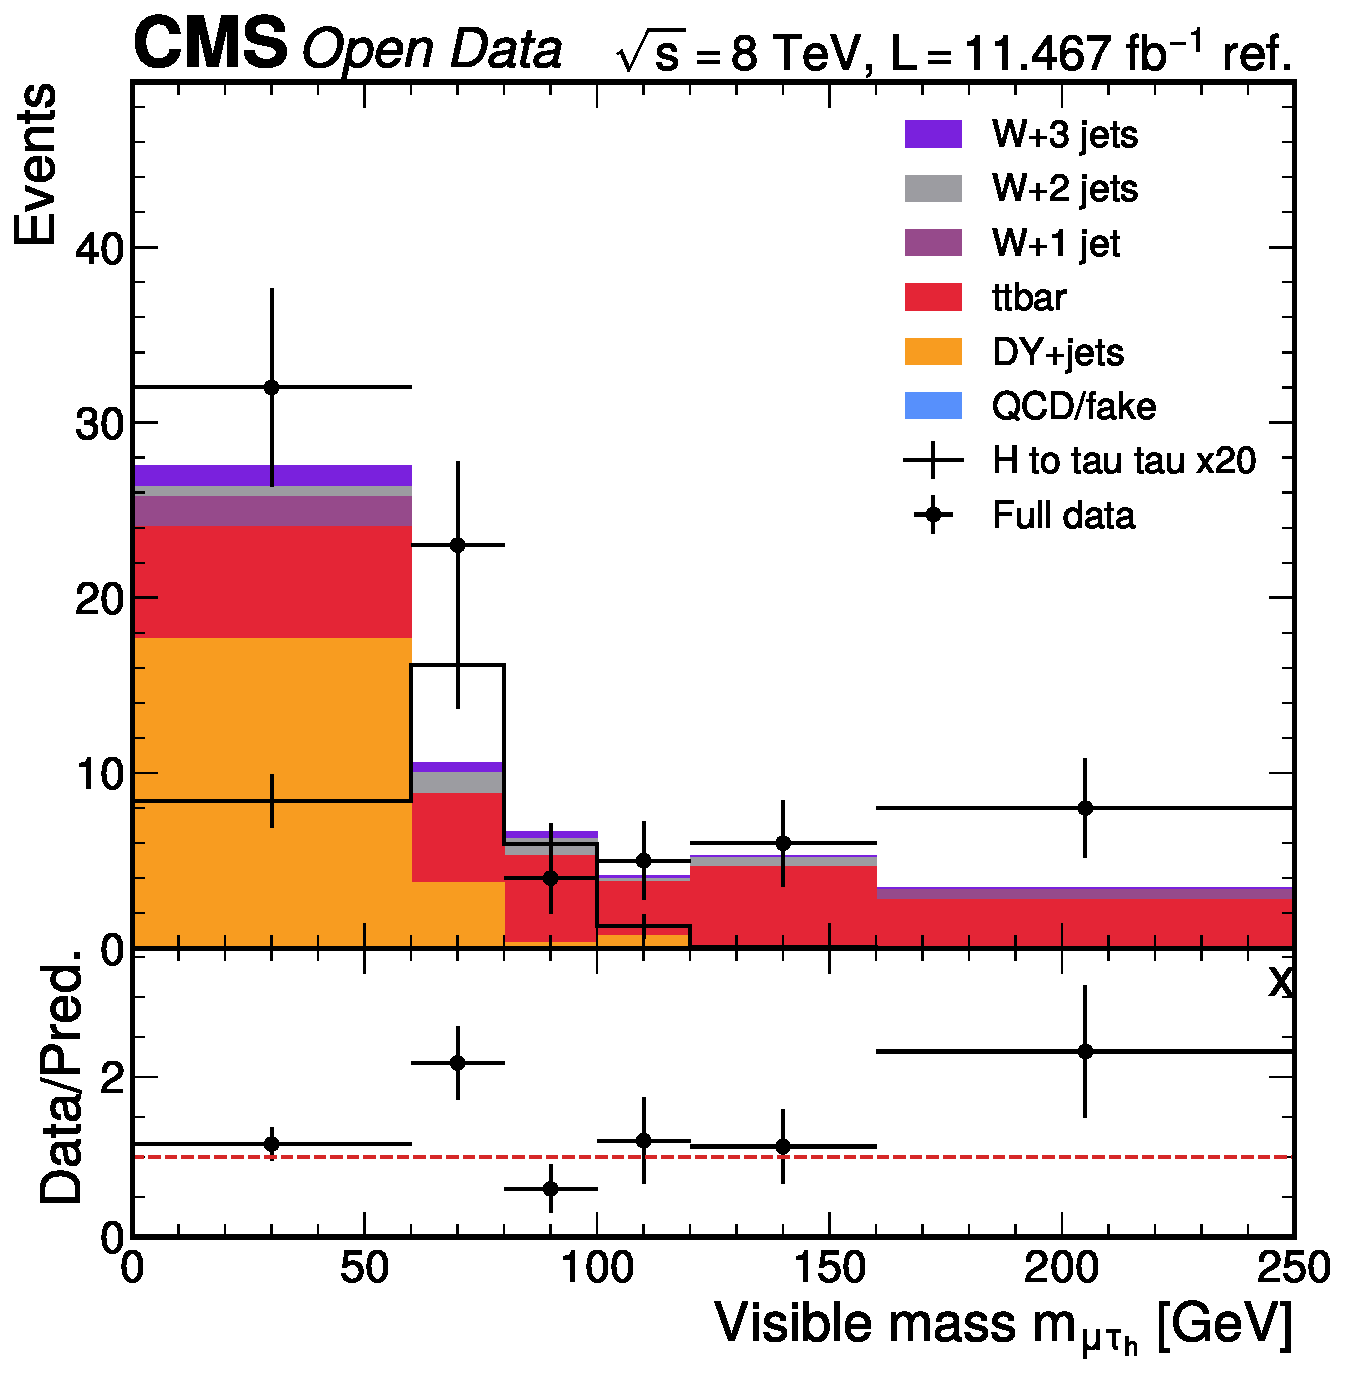
\includegraphics[height=0.35\textheight,width=\linewidth,keepaspectratio,alt={Visible-mass cross-check in the VBF category. This figure retains the visible-mass observable used in the conservative fallback analysis. It is shown as a validation cross-check for the primary calibrated-score result.}]{figures/observed_visible_vbf.pdf}}
\caption{Visible-mass cross-check in the VBF category. This figure
retains the visible-mass observable used in the conservative fallback
analysis. It is shown as a validation cross-check for the primary
calibrated-score result.}\label{fig:p4c-visible-vbf}
\end{figure}

\needspace{0.4\textheight}
\begin{figure}[htbp]
\centering
\pandocbounded{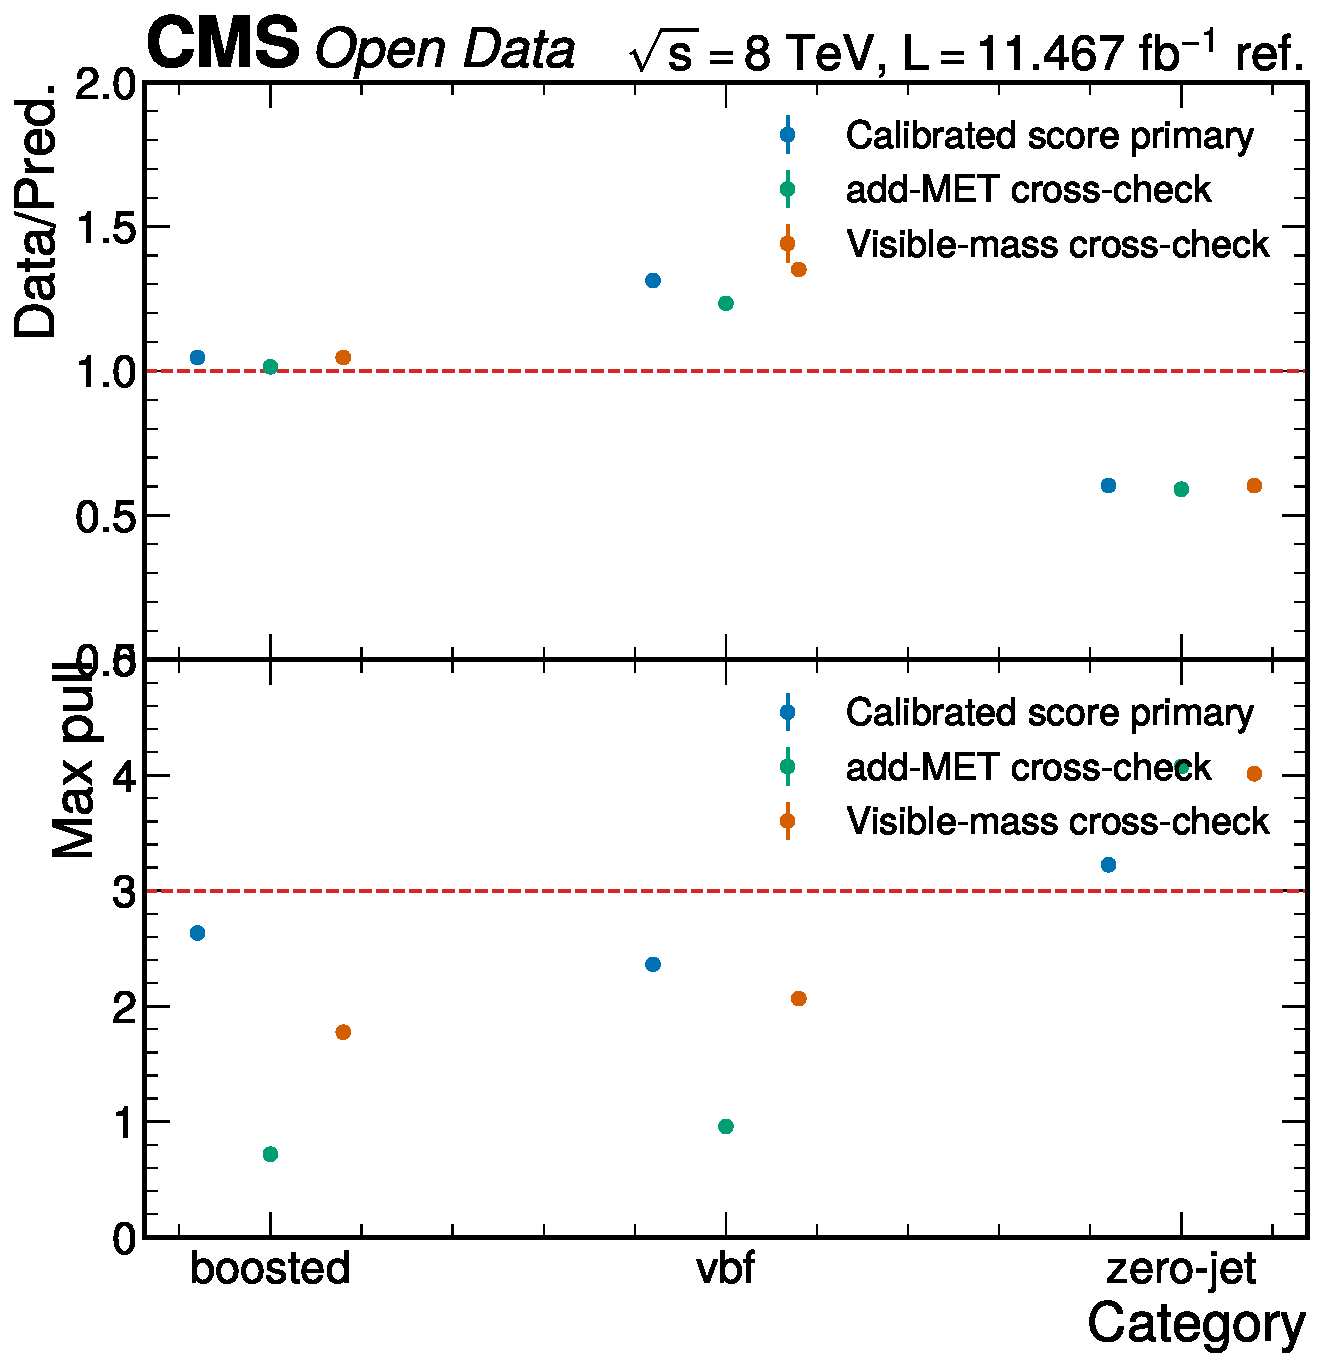
\includegraphics[height=0.35\textheight,width=\linewidth,keepaspectratio,alt={Observed pull and ratio summary. The figure compares the primary calibrated score and cross-check validation behavior after the QCD/fake, DY/Z, and input reweighting corrections. It is the central diagnostic for the final model choice.}]{figures/observed_pull_ratio_summary.pdf}}
\caption{Observed pull and ratio summary. The figure compares the
primary calibrated score and cross-check validation behavior after the
QCD/fake, DY/Z, and input reweighting corrections. It is the central
diagnostic for the final model choice.}\label{fig:p4c-pulls}
\end{figure}

\needspace{0.4\textheight}
\begin{figure}[htbp]
\centering
\pandocbounded{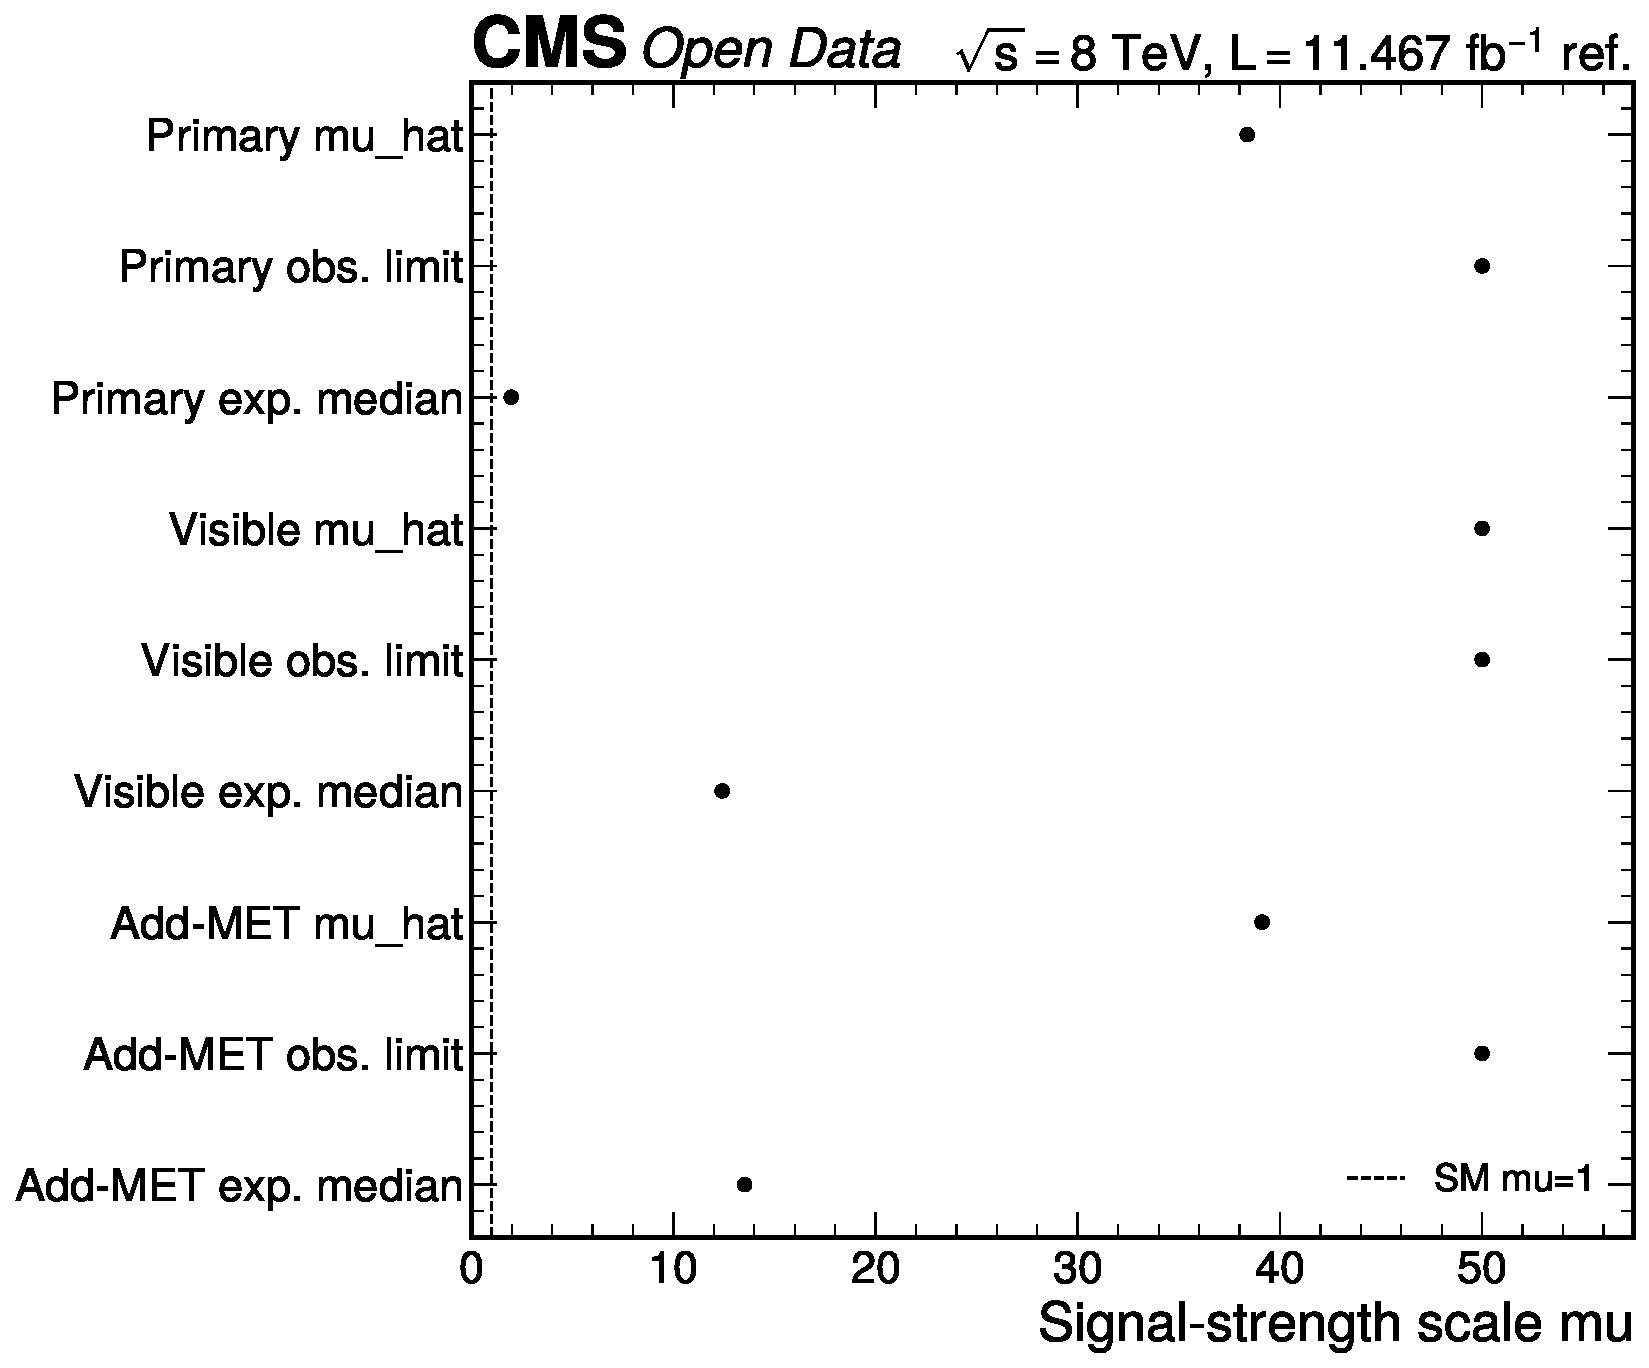
\includegraphics[height=0.35\textheight,width=\linewidth,keepaspectratio,alt={Observed limit and significance summary. The figure shows the primary calibrated-score fit and the cross-check fits on the same signal-strength scale. The result remains an Open Data diagnostic rather than CMS-quality evidence.}]{figures/observed_limit_significance_summary.pdf}}
\caption{Observed limit and significance summary. The figure shows the
primary calibrated-score fit and the cross-check fits on the same
signal-strength scale. The result remains an Open Data diagnostic rather
than CMS-quality evidence.}\label{fig:p4c-result-summary}
\end{figure}

\needspace{4\baselineskip}
\subsection{Phase 5 Obligation}\label{phase-5-obligation}

Phase 5 must report the calibrated-score plus QCD model as the final
observed result, while documenting the pre-training input reweighting,
the widened DY/Z normalization, and the absence of embedded/EWK Z
reduced samples. It must also state that the localized reduced mirror
has about 10\% of the Open Data record entries, while the 11.467/fb
value remains the cited normalization reference for these reduced
tutorial samples.
\clearpage

\needspace{4\baselineskip}
\section*{References}\label{references}
\addcontentsline{toc}{section}{References}

\end{document}
